\chapter{绪论}
\label{chp:introsuction}
\nomtypeG{ASP}{Answer Set Programming}{回答集程序}
\nomtypeG{GDPR}{General Data \\Protection Regulation}{通用数据保护准则}
\nomtypeG{DARPA}{Defense Advanced\\ Research Projects Agency}{美国国防部\\高级研究计划局}
\nomtypeG{ABA}{Assumption-based Argumentation}{基于假设的论证}
\nomtypeG{LABAS}{Labelled ABA-based Answer Set}{有标签的基于ABA的回答集}
\nomtypeG{NAF}{Negation As Failure}{失败即否定}
\nomtypeG{NLP}{Normal Logic Program}{一般逻辑程序}
\nomtypeG{IDE}{Integrated Development Environment}{集成开发环境}


\section{研究背景与动机}
随着人工智能技术的高速发展,基于人工智能技术的解决方案正在被各行各业普遍应用。与此同时,人工智能所做出的决策是否合法合规、值得信赖的问题引发人们的探讨,对人工智能可解释性的研究开始受到国内外的广泛关注。2021年3月,十三届全国人大四次会议通过《中华人民共和国国民经济和社会发展第十四个五年规划和2035年远景目标纲要》\cite{guowuyuan2021shisiwu},其中科技前沿领域攻关目标中提出了新一代人工智能学习推理与决策创新的要求;2017年10月,国务院印发的《新一代人工智能发展规划》\cite{guowuyuan2017aiplan}中更具体地指出要进一步研究不确定性推理与决策,机器直觉推理与因果模型等基础理论,同时提出了实现具备高可解释性、强泛化能力的人工智能的目标。2016年10月,美国DARPA实验室启动可解释的人工智能(eXplainableAI,XAI)项目\cite{gunning2017explainable} ,提出建立一套改进的机器学习技术生成可解释的模型,结合有效的解释技术,使得最终用户能够理解人工智能系统的目标;欧盟在2016年颁布的通用数据保护规范(GDPR\cite{regulation2016regulation} )中提出,“任何人都有权利拒绝接受仅基于机器处理得到的涉及重大个人利益的决策”,所有决策只有具备解释才会为人接受\cite{goodman2017european}。由此可见,解释在人工智能领域研究中越来越受到关注。

回答集编程(Answer Set Programming,ASP)是一种流行的用于决策和解决问题的人工智能编程范式。作为一种声明式语言,ASP程序作为具有强大的表达力,并已被成功用于多个领域\cite{erdem2016applications},例如生物学\cite{erdem2015generating}、心理学\cite{psychology2010Balduccini}、医学\cite{bao2011medical, zhang2014preliminary}、机器人家庭服务\cite{jjm2010robertasp}以及音乐创作\cite{boennAutomaticMusicComposition2011}等。使用ASP求解问题的主要优势是程序编写结构紧凑,编写速度很快,程序员可以专注于对问题的描述而不必关心搜索算法的具体设计,搜索求解的工作统一由各种求解器完成\cite{brain2008answer}。然而,这一优势的背后意味着ASP程序的推理求解对使用者而言是一个“黑盒”\cite{huaqi2018lp}。在求解过程中,用户无法得知答案是如何一步步推理得到的。当求解结果与个人认知不一致时,需要对推理结果进行完整、准确的解释。因此,有必要建立一个面向ASP程序的解释模型。另一方面,从ASP编程人员的角度看,当程序执行结果与预期不一致时,为了明确程序编写中是否存在问题,需要对程序进行调试。现有的实际应用中,对ASP程序进行调试通常是采用人工对程序中的规则和文字逐一检查的方式进行的,这一过程耗费了大量时间和精力\cite{dodaroInteractiveDebuggingNonground2015}。当程序规模不断增大时,调试的难度也随之上升。而在命令式编程语言(如Python,Java,C++等)中,通过设置断点、单步调试、观察变量值等与用户交互的调试方式,可以有效地发现程序中的问题\cite{stumptner1998survey}。在ASP程序的编写和调试中引入这种调试模式,辅助检查ASP程序中的语法和语义错误,能够有效降低ASP程序的学习门槛,节约开发过程中的时间成本,有助于推广ASP程序在工程中更广泛的应用。

综上,设计实现一个可交互的ASP程序解释和调试系统,在提升决策可解释性,增强开发效率方面具有重要的工程研究价值。本文针对上述对ASP程序进行解释和调试的实际需求,首先构建ASP程序解释模型,并基于该解释模型提出ASP程序的调试模型,在解释和调试模型的基础上,设计实现一个面向用户的交互式ASP程序解释和调试系统。
\section{相关研究现状}
当前,对ASP程序的解释,国内外的研究可分为对一致性ASP程序的解释和非一致性ASP程序的解释。其中,对一致性ASP程序的解释,也称为理由(justification),对非一致性ASP程序的解释,现有研究中认为就是ASP程序的调试(debugging)\cite{fandAnsWhy2019}。因此本节按照上述分类,分两部分介绍当前国内外研究现状。

\subsection{对一致性ASP程序的解释}
对一致性ASP程序的解释,按照解释呈现的形式又可以分为三类:基于文字与规则依赖图的解释,基于命题公式的解释和基于规则集的解释。Pontelli等人在\cite{pontelli2006justifications, pontelli2009justifications}中提出了离线解释(Off-line Justification)的概念。离线解释是描述某一回答集下原子真值的推导过程的图结构,其中每个顶点代表一个原子,每个边代表其连接的两个原子通过程序中某个规则形成的关联,由规则头部原子指向体部中的某个原子。花琪等人参考已有的关于ASP程序的图表示的方法\cite{albrecht2014construction,linke2005suitable},定义了以与或图为基础的ASP程序解释空间\cite{huaqi2018lp},该空间以程序中的规则与文字作为结点,通过边来表示其之间的依赖关系,最终将某一文字推理解释定义为解释空间的无环子图。这种解释方式与离线解释的最大不同在于将规则显式地引入了图中,而不仅是表示文字之间的依赖关系。可以看到,无论是否包含规则结点,上述解释中,使得某文字为真的每一步推导都包含在解释图中。与这种方式不同,Schulz等人基于论证(argumentation)理论提出LABAS解释\cite{schulz2013argumentationbased,schulz2016justifying},将推导中使用到的中间规则抽象出来,只展示待解释的文字以及推导过程中的出现的事实与规则的负体部,同时对否定文字$not\ l$的真值解释不再基于假设,而是通过对其肯定形式$l$的真值进行解释来呈现。除了上述两种由程序与回答集直接构建文字-规则依赖图的解释方式外,Cabalar等人还提出了基于因果推理的因果解释图,并在一系列工作中分别实现了不含失败即否定(Negation As Failure,NAF)文字的一般逻辑程序(Normal Logic Program,NLP)、含有NAF的NLP以及头部含有认知析取的逻辑程序的因果图解释\cite{albrecht2014construction,cabalar2016justificationsa,cabalar2017enablers}。由于因果推理本身就是一种形式化的推理方法,因此这种方式的解释能够很好地将推理过程中的语义信息在解释图中呈现。每一个回答集中的文字都对应着一个因果值集合,用于解释回答集包含该文字的原因。不同于基于图的解释,Carlos等人采用了声明式逻辑方法,基于良基模型(Well-founded Model)对NLP中原子的真值进行解释,最终以命题公式的形式呈现,被称为why-not解释\cite{viegasdamasio2013justifications}。除此之外,Bertaix等人从规则的角度出发研究逻辑程序解释的概念,其研究认为回答集计算中的固有猜测应当是针对规则的适用性进行猜测,而非原子真值。因此,其解释呈现的形式为一系列规则组成的集合\cite{beatrix2016justifications}。除了上述从规则和(或)文字的角度进行解释的方法以外,还有少部分研究着眼于证明的形式化的理论\cite{denecker1993justification,denecker2015formal}。在这种理论下,每个程序都引入了一种“证明框架”的语义结构,用于说明该程序某结论正确的潜在原因。不过,与综述的其他方法不同,这些工作侧重于将证明的概念作为数学工具来理解不同的语义(并提出新的语义),而不是以一种紧凑的方式来回答为什么一个逻辑程序能够得出某结论。表\ref{tbl:review_exp}总结了上述文献中的各种对一致性程序的解释方法及相关解释示例,并对应给出了本文所提出的解释的各要素说明。要说明的是,表中所有的示例均基于下面的程序$P_1$:
$$r_1: p \leftarrow t \land not\ q \qquad\qquad r_2: q \leftarrow s \qquad\qquad r_3: s \leftarrow not\ p \qquad\qquad r_4: t$$%
该程序有两个回答集,$M_1=\{t,s,q\}$,$M_2=\{t, p\}$。表\ref{tbl:review_exp}中的样例展示的是文字$p$在回答集$M_2$下的解释。可以看到,本文的解释在支持的程序类型、推导过程的展示、对否定文字的解释方式上均进行了改进。同时,在解释中考虑了非实例化程序的实例化处理,在推导过程的展示以及对否定文字的解释中还引入了用户交互。
\begin{sidewaystable}
    \caption{已有一致性程序解释工作总结与本文对比}\label{tbl:review_exp}
    \begin{adjustbox}{scale=0.55,center}
    \centering
    \semiLarge
    \setlength{\tabcolsep}{3mm}{
    \begin{tabular}{ m{0.15\textwidth}  m{0.15\textwidth}  m{0.1\textwidth} m{0.1\textwidth}  m{0.15\textwidth} m{0.12\textwidth}  m{0.1\textwidth} m{0.1\textwidth}  m{0.15\textwidth} m{0.25\textwidth}  }
      \hline
      \makecell{\textbf{解释方法}} & \makecell{\textbf{程序类型}} & \makecell{\textbf{解释角度}} & \makecell{\textbf{推导过程}} & \makecell{\textbf{解释对象}} &\makecell{\textbf{使用的}\\\textbf{其他模型}\footnote[1]{除稳定模型语义外的模型}} & \makecell{\textbf{否定文字}} & \makecell{\textbf{无限解释}} & \makecell{\textbf{无穷多个解释}} & \makecell{\textbf{解释结果示意}\\\textbf{(以}$P_1$\textbf{为例)}} \\ \hline
      \makecell{\textbf{离线解释}\cite{pontelli2006justifications,pontelli2009justifications}} & \makecell{NLP} & \makecell{文字依赖} & \makecell{完全包含} &\makecell{文字是否\\在回答集} & \makecell{良基语义} & \makecell{假设或进\\一步解释} & \makecell{有限程序\\不会出现} & \makecell{有限程序\\不会出现} &  \makecell{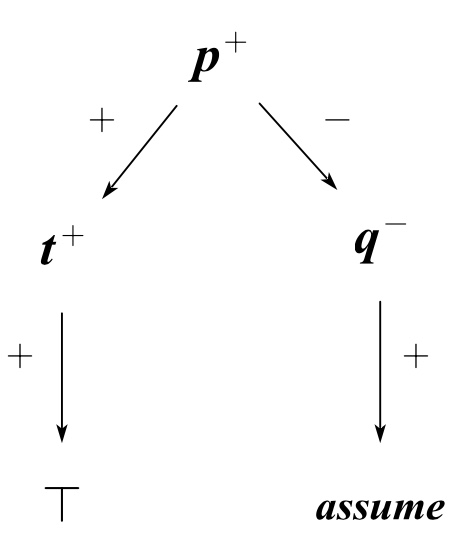
\includegraphics[scale=0.25,trim=0 0 0 -5]{figures/exp_1.jpg}}\\ 
      \makecell{\textbf{LABAS解释}\cite{schulz2013argumentationbased,schulz2016justifying}} & \makecell{含强否\\定的NLP} & \makecell{文字依赖} & \makecell{部分包含} &\makecell{文字是否\\在回答集} & \makecell{-} & \makecell{进一步解释} & \makecell{存在} & \makecell{存在} &  \makecell{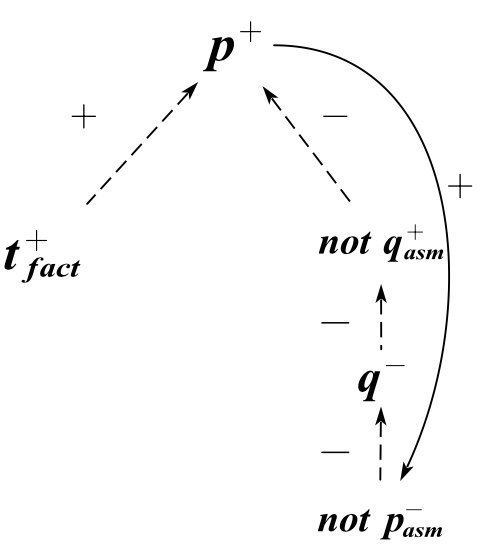
\includegraphics[scale=0.25,trim=0 0 0 -5]{figures/exp_2.jpg}}\\
      \makecell{\textbf{因果图解释}\cite{albrecht2014construction,cabalar2016justificationsa,cabalar2017enablers}} & \makecell{含强否定与\\嵌套表达式\\的NLP} & \makecell{规则-文字\\依赖} & \makecell{完全包含} &\makecell{文字在\\回答集} & \makecell{-} & \makecell{基于假设} & \makecell{有限程序\\不会出现} & \makecell{有限程序\\不会出现} &  \makecell{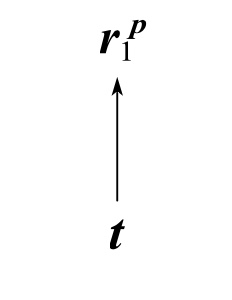
\includegraphics[scale=0.25,trim=0 0 0 -5]{figures/exp_3.jpg}}\\
      \makecell{\textbf{基本解释}\cite{huaqi2018lp}} & \makecell{NLP} & \makecell{规则-文字\\依赖} & \makecell{完全包含} &\makecell{文字在\\回答集} & \makecell{-} & \makecell{未做解释} & \makecell{有限程序\\不会出现} & \makecell{有限程序\\不会出现} &  \makecell{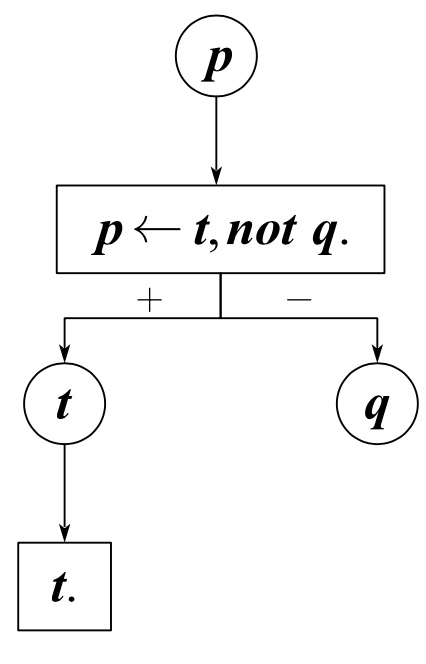
\includegraphics[scale=0.25,trim=0 0 0 -5]{figures/exp_4.jpg}}\\
      \makecell{\textbf{why-not解释}\cite{viegasdamasio2013justifications}} & \makecell{NLP} & \makecell{规则依赖} & \makecell{完全包含} &\makecell{文字是否属于\\完全良基模型} & \makecell{无需回答集} & \makecell{进一步解释} & \makecell{有限程序\\不会出现} & \makecell{有限程序\\不会出现} &  \makecell{$r_1 \land t \land\ not(q) \land \lnot r_3$} \\[5ex]
      \makecell{\textbf{基于规则解释}\cite{beatrix2016justifications}} & \makecell{NLP} & \makecell{规则依赖} & \makecell{完全包含} &\makecell{文字是否\\在回答集} & \makecell{-} & \makecell{进一步解释} & \makecell{有限程序\\不会出现} & \makecell{有限程序\\不会出现} &  \makecell{$\{r_1,t\}$}\\[5ex]
      \makecell{\textbf{形式理论解释}\cite{denecker1993justification,denecker2015formal}} & \makecell{NLP} & \makecell{文字依赖} & \makecell{完全包含} &\makecell{整个回答集} & \makecell{-} & \makecell{进一步解释} & \makecell{存在} & \makecell{有限程序\\不会出现} &  \makecell{$p \rightarrow t$\\$p \rightarrow not\ q \rightarrow not\ s \rightarrow p \rightarrow \ldots$}\\[5ex]
      \makecell{\textbf{本文}} & \makecell{含强否定的\\非实例化\footnote[2]{上述其他研究均未考虑对程序实例化的处理}\\NLP} & \makecell{规则-文字\\依赖} & \makecell{通过交互\\部分呈现} &\makecell{文字是否\\在回答集} & \makecell{良基语义} & \makecell{通过交互\\进行解释} & \makecell{有限程序\\不会出现} & \makecell{有限程序\\不会出现} &  \makecell{详见后文\\实验结果}\\
      \hline\\
    \end{tabular}}
\end{adjustbox}
\end{sidewaystable}
\subsection{对不一致ASP程序的调试}
对于不一致的 ASP 程序,现有的调试技术主要有如下三种类别:基于标签(元程序)技术、基于诊断技术和基于依赖图的方式\cite{dfj2012jiyuqifash}。前两种技术给出造成程序不一致的集合,但不能够清晰地体现集合之间的关系,以及错误产生的底层原因。第三种方法是基于支撑原因分析图的调试方法,该方法不仅可以以图的形式直观地给出程序中的错误,还可以给出错误来源及其相互间联系,从而为ASP程序调试提供更为强大的支撑。

Brain等人从Lin等人给出的\cite{lin2004assat}、由Jooyung Lee等人进一步扩展\cite{lee2005modeltheoretic}得到的回答集的定义角度出发,通过找到违背定义中的某一条原则,为程序$P$的每条规则的满足与不满足情况进行元程序规则的编写,能够用于说明某一原子为何不在一个一致性程序的回答集中,也能够用于为不一致程序生成潜在的回答集并指出为何该回答集不能满足程序的规则,进而解释程序不一致的原因,这一工作最终被集成在\textsf{SPOCK}平台中\cite{brain2007that,brain2007debugging}。\textsf{SPOCK}在调试中未能处理非实例化的问题,因此在\textsf{SPOCK}的基础上,Ostsch等人开发了能够处理包含变量的扩展逻辑程序的调试工具\textsf{Ouroboros}\cite{oetsch2010catching}。Polleres等人进一步扩展\textsf{Ouroboros}\cite{polleres2013debugging}来处理程序中的选择规则、基数以及弱约束\cite{calimeri2020aspcore2},最终由Fr\"uhst\"uck等人将该上述工作整合进入ASP集成开发环境(Integrated Development Environment,IDE)中,称为SeaLion IDE\cite{fruhstuck2013debugging}。

上述一系列工作存在一个显著的问题,调试生成的符号信息在数量上可能会非常庞大。\textsf{Ouroboros}通过要求用户声明一个意向的回答集来缩减规模,但对于不一致程序而言,用户可能无法声明出这样一个回答集。于是,第二类调试技术——引入用户交互的调试应运而生,这一系列技术提出诊断(diagnosis)的概念。其中Shchekotykhin在\textsf{SPOCK}的基础上通过询问逐个用户某一原子是否应该出现在回答集中并根据用户的答案缩减调试的规模,同时减少用户声明整个回答集的负担\cite{shchekotykhin2015interactive}。Dodaro\cite{dodaro2015interactive}和Gasteiger\cite{gasteiger2016integrated}在此基础上,实现了对于非实例化程序的调试,通过计算无法满足核心(unsatisfiable core),基于ASP求解器WASP\cite{alviano2013wasp,alviano2015advances}的求解过程来寻找程序的不一致性所在。

最后一类调试技术以Oetsch和P\"uhrer等人的一系列工作为代表\cite{oetsch2011stepping,oetsch2018stepwise,puhrer2014stepwise},以抽象约束程序为基础,对ASP程序使用类似于调试过程性语言程序的方式进行调试,该系统称为\textsf{Stepping}。与过程性语言程序调试不同的地方是,对于过程性语言,其程序执行的步骤在程序编写结束后就能够确定。然而由于声明式语言的特性,ASP程序的调试中,这一步骤并不是确定的。这样的过程实际上是一个尝试在与用户的交互中,使用户能够深入回答集计算的过程,不同于前面的调试方法,这种方法不规定用户指定一定正确的事实或规则,在未知任何条件的情况下, 用户可以从任何一条规则开始进行回答集计算的尝试。表\ref{tbl:review_dbg}中展示了已有程序调试工作总结与本文对比。可以看到,本文的调试基于本文定义的解释模型,同时用户可以按照调试命令式语言的方式,观察各原子真值、各规则适用性,指定规则适用的选择。

\begin{sidewaystable}
    \caption{已有程序调试工作总结与本文对比}\label{tbl:review_dbg}
    \begin{adjustbox}{scale=0.58,center}
    \centering
    \Large
    \setlength{\tabcolsep}{3mm}{
    \begin{tabular}{  m{0.2\textwidth}  m{0.2\textwidth} m{0.2\textwidth}  m{0.2\textwidth} m{0.2\textwidth}  m{0.2\textwidth} m{0.2\textwidth} m{0.2\textwidth}  }
      \hline
      \makecell{\textbf{调试方法}} & 
      \makecell{\textbf{程序类型}} & 
      \makecell{\textbf{是否可调试}\\\textbf{非实例化}} & 
      \makecell{\textbf{附加语法结构}\footnote[1]{包括选择规则、弱约束等}} & \makecell{\textbf{是否可解释}\\\textbf{一致性程序}}&
      \makecell{\textbf{是否需要}\\\textbf{指定回答集}} & 
      \makecell{\textbf{错误类型}} & 
      \makecell{\textbf{用户交互}} \\ \hline
      \makecell{\textbf{\textbf{SPOCK}}\cite{brain2007debugging,brain2008answer}} & 
      \makecell{NLP} & 
      \makecell{否} & 
      \makecell{否}&
      \makecell{是}&
      \makecell{可指定\\但不必须}&
      \makecell{不满足规则\\无支持原子\\无基原子}&
      \makecell{可能但\\不必须} \\[8ex]
      \makecell{\textbf{Ouroboros}\cite{oetsch2010catching}} & 
      \makecell{含否定的NLP} & 
      \makecell{是} & 
      \makecell{算术表达式\\大小比较}&
      \makecell{否}&
      \makecell{必须}&
      \makecell{不满足规则/约束\\无基原子}&
      \makecell{必须指定\\一个回答集}\\[8ex]

      \makecell{\textbf{DWASP}\cite{dodaro2015interactive}} & 
      \makecell{LP} & 
      \makecell{是} & 
      \makecell{否}&
      \makecell{否}&
      \makecell{可指定\\但不必须}&
      \makecell{最小无法\\满足核心}&
      \makecell{必须参与}\\[8ex]
      \makecell{\textbf{stepping}\cite{oetsch2011stepping,puhrer2014stepwise,oetsch2018stepwise}} & 
      \makecell{LP} & 
      \makecell{是} & 
      \makecell{聚合函数\\权重约束\\外部原子}&
      \makecell{是}&
      \makecell{间接需要\\但不必须}&
      \makecell{规则无法满足性\\原子间真值矛盾}&
      \makecell{必须参与}\\[8ex]
      \makecell{\textbf{DWASP}\cite{dodaro2015interactive}} & 
      \makecell{LP} & 
      \makecell{是} & 
      \makecell{否}&
      \makecell{否}&
      \makecell{可指定\\但不必须}&
      \makecell{最小无法\\满足核心}&
      \makecell{必须参与}\\[8ex]
      \makecell{\textbf{可交互SPOCK}\cite{shchekotykhin2015interactive}} & 
      \makecell{LP} & 
      \makecell{否} & 
      \makecell{否}&
      \makecell{否}&
      \makecell{可指定\\但不必须}&
      \makecell{不满足规则\\无支持原子\\无基原子}&
      \makecell{必须参与}\\[8ex]
      \makecell{\textbf{本文}}& 
      \makecell{LP} & 
      \makecell{是} & 
      \makecell{聚合函数\\权重约束\\外部原子}&
      \makecell{是}&
      \makecell{可指定\\但不必须}&
      \makecell{基于解释模型\\的调试模型}&
      \makecell{必须参与\\可自行结束}\\[8ex]
      \hline\\
    \end{tabular}}
\end{adjustbox}
\end{sidewaystable}

\subsection{研究现状不足}
Gilpin等人指出,人工智能中的解释可以从两个角度评价:第一个是可解释性(interpretability),即生成一个简单、有意义且为人所接受的解释;第二个是完整性(completeness),即在解释系统中详尽地阐明得到结果经过的操作。而同时达到上述两个标准,是当今人工智能可解释问题的一个挑战\cite{gilpin2018explaining}。这一挑战在现有的ASP程序解释中体现在解释的简洁性与清晰性难以达到平衡。考虑下面的程序$P_2$:
\begin{align}
    &r_1:\quad m(i+1) \leftarrow m(i), p(i).\ \ \  \mathit{for}\ i \in \{1, \ldots, k\} \notag\\ 
    &r_2:\quad m(j+1) \leftarrow n(j), p(j).\ \ \  \mathit{for}\ j \in \{1, \ldots, k\} \notag\\
    &r_3:\quad m(i) \leftarrow p(i).\ \ \  \mathit{for}\ i \in \{1, \ldots, k\}  \notag\\
    &r_4:\quad n(j) \leftarrow p(j).\ \ \  \mathit{for}\ j \in \{1, \ldots, k\} \notag
  \end{align}
当给定事实$F=\{m(1), m(k), n(1), \ldots n(k),p(1), \ldots p(k)\} (k \ge 2$且$k$为常数),程序$P_2 \cup F$的唯一回答集为$\{m(1), \ldots m(k+1), n(1), \ldots n(k), p(1), \ldots p(k)\}$。当$k=2$时,对于$m(2)$在回答集中的原因,可以解释为$\{m(2)\}$本身是事实;也可以解释为$\{p(1)\}$作为事实成立,再由$r_3$推导得到;又可以解释为$\{m(1),p(1)\}$作为事实成立,再由$r_1$推导得到;还可以解释为$\{n(1),p(1)\}$作为事实成立再由$r_2$推导得到。当$k$不断增大,可选择的解释规模将呈现指数级增长,这在基于依赖图的解释中体现为图的结点与边过于复杂,在基于命题符号的解释中则会输出大量复杂的符号表示,\textbf{解释均不具有可读性};另一方面,部分解释为了追求简洁性,省略中间结论,只展示最直接的文字间的依赖(离线解释,LABAS)。例如上面的程序中,认为$m(k)$成立就是基于事实,而忽略了其他支持$m(k)$成立的证据,\textbf{解释的完整性无法得到保证}。

本文在处理解释的过程中,采用引导用户逐层展开的思想,对每一个文字或规则结点可能展开的方向进行预判,并提示用户根据个人的意愿以树状形式扩展得到解释。这一思想进一步被用于调试模型中,以提高用户在调试过程中的参与度,最大程度还原命令式程序的调试过程,发挥其易操作、交互性好的优势,提升ASP程序的调试效率。
\section{研究目标与内容}
本课题的主要目标是研究并设计针对ASP程序的解释模型与调试模型,实现一个针对ASP程序的解释与调试系统。其中ASP解释模型为ASP调试模型的设计提供了基础,两模型共同为解释与调试系统的设计与实现提供了核心方法,最终通过实例验证本系统的科学性和有效性。具体研究内容如下:
\begin{enumerate}[label=(\arabic*),topsep=0pt]
    \setlength\itemsep{-0.3em}
    \item \textbf{ASP程序解释模型的设计。}首先给出某文字在一致性ASP程序下解释的定义,根据该定义设计解释生成算法。对非实例化程序,研究面向解释的ASP程序实例化方法。
    \item \textbf{ASP程序调试模型的设计。}在解释模型的基础上,研究导致不一致ASP程序的原因,进一步定义不一致ASP程序的调试模型;根据调试的定义,设计调试算法。
    \item \textbf{设计实现ASP程序的调试和求解结果解释的平台。}面向实例应用,对外部函数、非实例化文字等ASP程序语法特性进行解释方案探索,在解释和调试模型的基础上,设计实现可交互非实例化ASP程序解释和调试系统,并对系统进行实验验证。
\end{enumerate}
\section{研究方法与技术路线}
本文在上述对相关工作的调查与研究的基础上,采用模型设计和理论研究相结合,系统实现和案例应用相结合,逐步递进,从设计到最终实现的研究方法。通过研究ASP程序的推理解释机制,构建面向用户的可交互ASP推理解释模型,并在此基础上结合命令式语言成熟的调试技术,以解释模型为基础设计ASP程序的调试模型,最终以两个模型为核心方法,设计实现ASP程序解释和调试系统,通过实际程序进行系统验证。
\begin{figure}[!ht] 
    \centering 
    \includegraphics[width=\linewidth]{figures/研究内容关联图.jpg}
    \caption{ASP程序解释与调试技术路线图} 
    \label{fig:1_1} 
\end{figure}
如图\ref{fig:1_1}所示,本项目的具体研究路线如下:
\begin{enumerate}[label=(\arabic*),topsep=0pt]
    \setlength\itemsep{-0.3em}
    \item 参考已有工作中对ASP程序进行推理解释的方法,首先给出一致性程序关于某文字解释的定义。针对已有工作中解释中规模较大、部分否定文字解释不清晰的问题,通过引入用户交互机制,有效缩减解释呈现的规模,提高获取解释的有效性。对于非实例化的ASP程序,研究当前实例化工具面向解释存在的局限性,提出一套基于元编程技术的用户交互下的实例化程序获取方案;
    \item 在解释模型的基础上,进一步定义 ASP 程序的调试。本课题中,对于一致性ASP程序,调试的主要思路是对ASP解释图进行的深度优先遍历。对于不一致 ASP 程序的调试,由于程序没有回答集,因此通过引导用户根据预期的回答集对暂不确定的文字-规则依赖图进行标记,根据用户的标记信息通过规则的可满足性自动计算文字-规则依赖图中各文字的真值,进而构建解释空间,直到发现真值的矛盾与程序中存在的问题;
    \item 基于ASP解释与调试模型,设计并实现ASP解释和调试系统,以验证本文所设计的两个模型的有效性。该系统的目标用户是具有ASP编程经验的ASP编程人员,以B/S架构为基础架构进行系统设计,分别实现前端与后端两个部分的功能。前端用于接受用户输入的ASP程序、待解释的文字、解释与调试过程中交互信息,并向后端传递这一交互结果,后端根据用户的反馈,主动进行后续交互或直接生成解释与调试结果。最后,通过几个ASP程序来展示系统对程序进行解释与调试的实际效果。
\end{enumerate}
\section{论文结构}
本文共分为六个章节,各章节主要内容具体如下: 

第一章为绪论,总体介绍本文的研究背景及意义、相关研究现状与不足、研究目标与研究内容、研究方法与技术路线及本文的结构安排。

第二章对ASP推理理论方法的背景知识进行介绍,具体包括ASP程序的语法、ASP程序的语义及ASP程序的求解器等。

第三章研究ASP程序解释模型,包括ASP程序解释的定义、交互解释的生成算法。在已有研究的基础上,使用图作为推理解释的表示方法,重点讨论如何将用户的选择引入解释中,形成用户友好、易于接受的解释模型,同时对非实例化程序提出一套面向解释的实例化方案。

第四章在ASP解释模型的基础上,进一步研究ASP程序调试模型。包括ASP程序调试的定义,以及根据该调试模型提出的调试算法。重点面向ASP语言作为声明式语言,在推导过程中原子推导顺序不确定造成调试困难的问题,通过交互引导用户进行选择,将命令式语言调试的风格引入声明式语言。

第五章介绍基于上述两个模型所设计实现的ASP程序解释和调试系统,主要包括系统设计、系统实现以及应用案例展示等,在系统实现中提出对非实例化程序、外部函数等非基本语法特性进行解释的探索。

第六章中对本文工作加以总结,并展望未来工作。